\documentclass[letterpaper]{article} % DO NOT CHANGE THIS
\usepackage[submission]{aaai2027}  % DO NOT CHANGE THIS
% The serif, sans-serif, and monospaced fonts are loaded automatically by
% aaai2027.sty (newtxtext, helvet, courier). DO NOT add \usepackage{times},
% \usepackage{helvet}, \usepackage{courier}, or any other font package.
\usepackage[hyphens]{url}  % DO NOT CHANGE THIS
\usepackage{graphicx} % DO NOT CHANGE THIS
\urlstyle{rm} % DO NOT CHANGE THIS
\def\UrlFont{\rm}  % DO NOT CHANGE THIS
\usepackage{natbib}  % DO NOT CHANGE THIS AND DO NOT ADD ANY OPTIONS TO IT
\usepackage{caption} % DO NOT CHANGE THIS AND DO NOT ADD ANY OPTIONS TO IT
\frenchspacing  % DO NOT CHANGE THIS
%
% These are recommended to typeset algorithms but not required. See the subsubsection on algorithms. Remove them if you don't have algorithms in your paper.
\usepackage{algorithm}
\usepackage{algorithmic}
\usepackage{enumitem}
%
% These are recommended to typeset listings but not required. See the subsubsection on listing. Remove this block if you don't have listings in your paper.
\usepackage{newfloat}
\usepackage{listings}
\DeclareCaptionStyle{ruled}{labelfont=normalfont,labelsep=colon,strut=off} % DO NOT CHANGE THIS
\lstset{%
	basicstyle={\footnotesize\ttfamily},% footnotesize acceptable for monospace
	numbers=left,numberstyle=\footnotesize,xleftmargin=2em,% show line numbers, remove this entire line if you don't want the numbers.
	aboveskip=0pt,belowskip=0pt,%
	showstringspaces=false,tabsize=2,breaklines=true}
\floatstyle{ruled}
\newfloat{listing}{tb}{lst}{}
\floatname{listing}{Listing}

%
% Recommended for better-looking tables
\usepackage{booktabs}

%
% Keep the \pdfinfo as shown here. There's no need
% for you to add the /Title and /Author tags.
\pdfinfo{
/TemplateVersion (2027.1)
}

% DISALLOWED PACKAGES
% \usepackage{authblk} - This package is specifically forbidden
% \usepackage{balance} - This package is specifically forbidden
% \usepackage{CJK} - This package is specifically forbidden
% \usepackage{float} - This package is specifically forbidden
% \usepackage{flushend} - This package is specifically forbidden
% \usepackage{fullpage} - This package is specifically forbidden
% \usepackage{geometry} - This package is specifically forbidden
% \usepackage{hyperref} - This package is specifically forbidden
% \usepackage{navigator} - This package is specifically forbidden
% (or any other package that embeds links such as navigator or hyperref)
% \usepackage{indentfirst} - This package is specifically forbidden
% \usepackage{layout} - This package is specifically forbidden
% \usepackage{multicol} - This package is specifically forbidden
% \usepackage{nameref} - This package is specifically forbidden
% \usepackage{savetrees} - This package is specifically forbidden
% \usepackage{setspace} - This package is specifically forbidden
% \usepackage{stfloats} - This package is specifically forbidden
% \usepackage{tabu} - This package is specifically forbidden
% \usepackage{titlesec} - This package is specifically forbidden
% \usepackage{tocbibind} - This package is specifically forbidden
% \usepackage{ulem} - This package is specifically forbidden
% \usepackage{wrapfig} - This package is specifically forbidden
% DISALLOWED COMMANDS
% \nocopyright - Your paper will not be published if you use this command
% \addtolength - This command may not be used
% \balance - This command may not be used
% \baselinestretch - Your paper will not be published if you use this command
% \clearpage - No page breaks of any kind may be used for the final version of your paper
% \columnsep - This command may not be used
% \newpage - No page breaks of any kind may be used for the final version of your paper
% \pagebreak - No page breaks of any kind may be used for the final version of your paper
% \pagestyle - This command may not be used
% \tiny - This is not an acceptable font size.
% \vspace{- - No negative value may be used in proximity of a caption, figure, table, section, subsection, subsubsection, or reference
% \vskip{- - No negative value may be used to alter spacing above or below a caption, figure, table, section, subsection, subsubsection, or reference

\setcounter{secnumdepth}{0} %May be changed to 1 or 2 if section numbers are desired.

% The file aaai2027.sty is the style file for AAAI Press
% proceedings, working notes, and technical reports.
%

% Title

% Your title must be in mixed case, not sentence case.
% That means all verbs (including short verbs like be, is, using,and go),
% nouns, adverbs, adjectives should be capitalized, including both words in hyphenated terms, while
% articles, conjunctions, and prepositions are lower case unless they
% directly follow a colon or long dash
\title{Is Retrieval All You Need? Assessment and Emergence of Novelty in Protein Structure Generation}
\author{
    %Authors
    % All authors must be in the same font size and format.
    Written by AAAI Press Staff\textsuperscript{\rm 1}\thanks{With help from the AAAI Publications Committee.}\\
    AAAI Style Contributions by Peter Patel Schneider,
    Sunil Issar,\\
    J. Scott Penberthy,
    George Ferguson,
    Hans Guesgen,
    Francisco Cruz\equalcontrib\corresponding,
    Marc Pujol-Gonzalez\equalcontrib\corresponding
}
\affiliations{
    %Afiliations
    \textsuperscript{\rm 1}Association for the Advancement of Artificial Intelligence\\
    % If you have multiple authors and multiple affiliations
    % use superscripts in text and roman font to identify them.
    % For example,

    % Sunil Issar\textsuperscript{\rm 2},
    % J. Scott Penberthy\textsuperscript{\rm 3},
    % George Ferguson\textsuperscript{\rm 4}\corresponding,
    % Hans Guesgen\textsuperscript{\rm 5}
    % Note that the comma should be placed after the superscript

    1101 Pennsylvania Ave, NW Suite 300\\
    Washington, DC 20004 USA\\
    % email address must be in roman text type, not monospace or sans serif
    proceedings-questions@aaai.org
%
% See more examples next
}

%Example, Single Author, ->> remove \iffalse,\fi and place them surrounding AAAI title to use it
\iffalse
\title{My Publication Title - Single Author}
\author {
    Author Name
}
\affiliations{
    Affiliation\\
    Affiliation Line 2\\
    name@example.com
}
\fi

\iffalse
%Example, Multiple Authors, ->> remove \iffalse,\fi and place them surrounding AAAI title to use it
\title{My Publication Title - Multiple Authors}
\author {
    % Authors
    First Author Name\textsuperscript{\rm 1,\rm 2}\equalcontrib,
    Second Author Name\textsuperscript{\rm 2}\equalcontrib,
    Third Author Name\textsuperscript{\rm 1}\corresponding
}
\affiliations {
    % Affiliations
    \textsuperscript{\rm 1}Affiliation 1\\
    \textsuperscript{\rm 2}Affiliation 2\\
    firstAuthor@affiliation1.com, secondAuthor@affilation2.com, thirdAuthor@affiliation1.com
}
\fi


\begin{document}

\maketitle

\begin{abstract}
Protein backbone generation models are increasingly capable of exploring novel fold space based on low full-chain structural similarity to known proteins. Yet a low full-chain similarity alone cannot tell whether a structure embodies a genuinely new fold or simply recombines familiar structural units into a globally novel arrangement. To quantify the extent of this recombination, we introduce the Domain Retrieval Rate (DRR), defined as the proportion of generated backbones whose constituent domains can be matched to known structures in CATH S40. Applied to six backbone generation models, including diffusion, flow-matching, and autoregressive paradigms, DRR reveals that the vast majority of outputs from high-designability models contain domains already present in known fold space, even when their full-chain structures appear novel. The gap between domain-level and full-chain retrievability provides a direct measure of how much apparent novelty is combinatorial rather than structural. To calibrate what retrieval alone can achieve, we propose RetFold, a zero-training baseline that constructs backbones by retrieving CATH domains and refining inter-domain connections through geometry-based helix-linker optimization. Without any GPU training, RetFold matches RFdiffusion in designability and full-chain novelty while generating backbones over 100 times faster, and it attains the highest designability and combinatorial novelty among all evaluated methods. Together, DRR and RetFold establish that full-chain structural novelty is insufficient evidence of fold-level innovation and that current generative performance is largely reproducible through retrieval and recombination of known domains. Future evaluation should decompose novelty across structural granularities and calibrate generative claims against retrieval-based lower bounds.
\end{abstract}

% Uncomment the following to link to your code, datasets, an extended version or similar.
% You must keep this block between (not within) the abstract and the main body of the paper.
% Make sure that you do not de-anonymize yourself with these links.
% \begin{links}
%     \link{Code}{https://aaai.org/example/code}
%     \link{Datasets}{https://aaai.org/example/datasets}
%     \link{Extended version}{https://aaai.org/example/extended-version}
% \end{links}

\section{Introduction}

Protein backbone generation models are increasingly claimed to explore fold space beyond known proteins. Recent generators spanning diffusion~\cite{watson2023novo,yim2023se}, flow matching~\cite{yim2023fast,campbell2024generative}, and autoregressive backbones~\cite{ingraham2023illuminating} report that substantial fractions of their outputs have no close structural match in existing databases, suggesting the invention of previously unseen folds. This claim rests on two pillars: generated backbones pass inverse-folding and structure-prediction validation~\cite{dauparas2022robust,abramson2024accurate}, confirming in-silico designability; and they exhibit low full-chain structural similarity to all entries in known protein structure databases, indicating apparent novelty. We argue that neither condition, alone or together, is sufficient to establish fold-level novelty, and that the gap between full-chain and domain-level novelty exposes a systematic overestimation of fold-level novelty in current protein structure generation models.

The core issue is a granularity mismatch. Full-chain comparison treats a generated backbone as a monolithic unit, yet natural proteins are modular: they are composed of several folding domains that recombine across evolution~\cite{chothia1992one,orengo1997cath}. A structure that concatenates two known domains in a previously unseen orientation will receive a low full-chain similarity score despite containing no new fold. This is combinatorial novelty, arising from the exponential space of multi-domain arrangements, not fold-level innovation within the finite and largely catalogued domain fold space~\cite{wolf2000estimating,levitt2009nature}. Conflating the two allows models that recombine known building blocks to appear as if they have expanded the universe of protein folds, when they have only explored new configurations within it.

A second confounding factor compounds this overestimation. Generated backbones that are physically implausible cannot match any known protein, so they automatically appear to be novel under full-chain comparison. If such non-designable structures are included in novelty statistics, models with lower structural quality will paradoxically report higher novelty rates. Designability filtering is therefore not merely a quality check but a logical prerequisite for novelty assessment: only backbones confirmed to encode foldable proteins~\cite{dauparas2022robust, abramson2024accurate} should enter the novelty denominator. Without this prerequisite, the two confounding factors operate jointly, with non-designable artifacts inflating the numerator and full-chain granularity obscuring domain-level reuse in the remainder.

\begin{figure*}[ht]
\centering
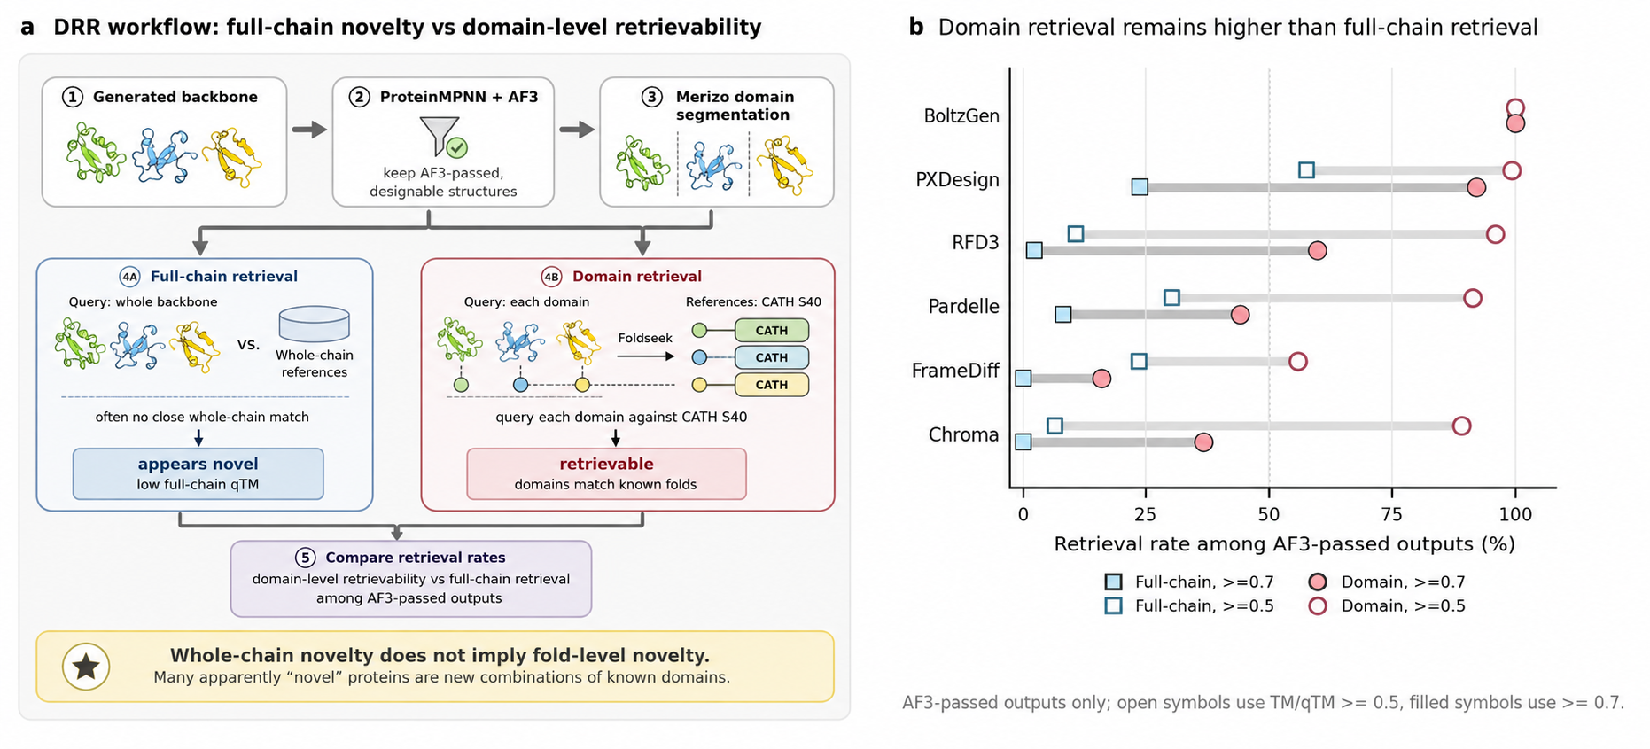
\includegraphics[width=\textwidth]{Figures/fig_intro_domain_retrievability_problem.pdf}
\caption{DRR workflow for separating full-chain novelty from domain-level retrievability. (a)~Generated backbones are first filtered by ProteinMPNN and AF3 to retain designable structures, then segmented into domains by Merizo. The same AF3-passed backbone is evaluated through two retrieval views: full-chain retrieval searches the intact backbone and may find no close whole-chain match, making the structure appear novel, whereas domain retrieval searches each Merizo domain against CATH S40 with Foldseek and can reveal that the constituent fold units are known. DRR compares these retrieval rates among AF3-passed outputs. (b)~Across six generation models, domain-level retrieval remains consistently higher than full-chain retrieval. Open symbols denote TM/qTM${\geq}0.5$ and filled symbols denote TM/qTM${\geq}0.7$ retrieval against CATH S40.}
\label{fig:intro_domain_retrievability}
\end{figure*}

Those two issues motivate a domain-centric evaluation framework. We introduce Domain Retrieval Rate (DRR), a metric that decomposes generated backbones into structural domains and measures the proportion whose constituent domains can be matched to known folds in the CATH S40 database~\cite{orengo1997cath}. By comparing domain-level retrievability against full-chain retrievability, DRR directly quantifies how much apparent novelty is combinatorial rather than structural. Figure~\ref{fig:intro_domain_retrievability} previews the central finding: across six generation models, domain-level retrieval remains high (86\%-99\% at TM$\geq 0.5$) even when full-chain retrieval varies widely, revealing that most designable outputs are assembled from known fold units regardless of whether the full-chain arrangement itself appears novel.

To calibrate what retrieval alone can achieve, we further propose RetFold, a zero-training baseline that constructs protein backbones by retrieving CATH domains and assembling them through geometry-based helix-linker optimization. RetFold requires no GPU training and no learned generative prior; it serves as a lower-bound calibrator for the field. If such a pipeline can match trained generators in designability, structural diversity, and topology coverage, then these metrics cannot distinguish learned generative capacity from retrieval and recombination. Empirically, RetFold achieves a 93\% AlphaFold3 pass rate, the highest designability and combinatorial novelty among all evaluated methods, and produces 97\% full-chain novel structures at 1.85 seconds per backbone, establishing that the performance envelope attributed to deep generative models is largely reproducible without learning.



% Protein structure generation has emerged as a central task in AI-driven protein design. Diffusion models, flow-matching models, and other deep generative approaches can produce protein backbones that pass sequence design and structure prediction validation, leading to the expectation that they explore previously unknown protein fold space. This claim is typically supported by two types of evidence: high designability under AlphaFold-based validation and low structural similarity to known proteins under full-chain alignment. However, whether such evidence is sufficient to establish genuine fold-level novelty remains an open question.

% A key limitation is that novelty is typically measured at the full-chain level. A generated structure is considered novel if no sufficiently similar full-chain match is found in known databases. This criterion conflates two fundamentally different sources of apparent novelty: a structure may contain genuinely new domain-level folding patterns, or it may simply be composed of known structural units in a non-natural arrangement. In the latter case, the structure appears novel under full-chain comparison even though its constituent domains are already well represented in existing databases. Recombining known domains is useful for protein engineering, but it should not be interpreted as evidence of new fold discovery.

% A second confounding factor is designability. Generated backbones that are physically implausible are unlikely to match any known structure. If such non-designable artifacts are included in novelty statistics, a model with poorer structural quality may appear more novel simply because its outputs do not correspond to stable conformations. Novelty assessment without designability filtering therefore systematically overestimates the creative capacity of generative models.

% Figure~\ref{fig:intro_domain_retrievability} illustrates this ambiguity directly. When we decompose generated backbones into structural domains and search each domain against the CATH database, the majority of AF3-passed (designable) structures remain highly retrievable at the domain level-even for models widely regarded as producing novel outputs. Meanwhile, AF3-failed structures must be excluded from novelty claims entirely.

% These observations motivate a domain-centric, multi-granularity evaluation. We introduce \textbf{Domain Retrieval Rate (DRR)}, a metric that quantifies the proportion of generated backbones whose constituent domains can be matched to known structures in CATH S40. By comparing domain-level and full-chain retrievability, DRR directly measures how much of a model's apparent novelty is combinatorial rather than fold-level.

% We further introduce \textbf{RetFold}, a zero-training retrieval-and-assembly baseline that tests how much of the observed designability and novelty can be achieved without training a generative model. RetFold constructs protein backbones by retrieving and assembling known CATH domains, serving as a lower-bound calibrator: if retrieval alone can match generative models in designability, diversity, and topology coverage, then full-chain novelty alone is insufficient evidence of genuine fold discovery.

In summary, the contributions are summarized as follows:
\begin{itemize}
\item We identify the granularity gap in current novelty evaluation and propose DRR, a domain-centric metric that quantifies how much of a model's output can be explained by known domain-level folds, separating combinatorial novelty from fold-level innovation.
\item We provide systematic empirical evidence, across six representative models spanning diffusion, flow-matching, and autoregressive paradigms, that full-chain novelty consistently overstates fold-level creative capacity.
\item We introduce RetFold, a zero-training retrieval-and-assembly baseline that matches or exceeds trained generators in designability, diversity, and topology coverage, establishing a practical lower bound.
\end{itemize}

\section{Related Work}

\subsection{Protein Backbone Generation}

Deep generative models for protein backbone design span several paradigms. Diffusion-based methods iteratively denoise residue-level coordinate frames: RFdiffusion applies structure-conditioned denoising over SE(3) frames for unconditional and motif-scaffolded generation~\cite{watson2023rfdiffusion}; FrameDiff formulates backbone generation as a diffusion process directly on residue rigid-body frames~\cite{yim2023framediff}; Chroma combines graph-neural-network denoising with programmable conditioning for large-scale backbone sampling~\cite{ingraham2023chroma}. Flow-matching approaches such as FrameFlow~\cite{yim2023frameflow} and FoldFlow-2~\cite{huguet2024foldflow2} provide continuous normalizing flows on SE(3) manifolds with improved sampling efficiency. Beyond diffusion and flow matching, ProtPardelle generates backbones autoregressively over residue frames~\cite{chu2024protpardelle}, BoltzGen uses Boltzmann generators to sample equilibrium backbone conformations~\cite{zheng2024boltzgen}, and PXDesign employs a structure-based inverse design framework~\cite{wang2024pxdesign}. These methods collectively represent the current landscape of protein backbone generators evaluated in this work.

% Protein backbone generation aims to sample three-dimensional backbone geometries that can be realized by amino-acid sequences and used as scaffolds for protein design. Existing methods span several generative paradigms. Diffusion-based methods iteratively denoise residue-level coordinate frames: RFdiffusion performs structure-conditioned denoising over SE(3) frames for unconditional and motif-scaffolded generation~\cite{watson2023rfdiffusion}; FrameDiff formulates backbone generation as diffusion directly on residue rigid-body frames~\cite{yim2023framediff}; and Chroma combines graph-neural-network denoising with programmable conditioning for large-scale backbone sampling~\cite{ingraham2023chroma}. Flow-matching methods, including FrameFlow~\cite{yim2023frameflow} and FoldFlow-2~\cite{huguet2024foldflow2}, define continuous normalizing flows on SE(3) manifolds to improve sampling efficiency. Other approaches explore autoregressive generation over residue frames~\cite{chu2024protpardelle}, Boltzmann-generator-based sampling of equilibrium backbone conformations~\cite{zheng2024boltzgen}, and structure-based inverse design~\cite{wang2024pxdesign}. 
% Despite these advances, evaluations based primarily on designability and full-chain novelty may not rule out the possibility that generated backbones are explained by retrieval and recombination of known domain-level folds. Our work therefore does not introduce another backbone generator; instead, it evaluates whether the novelty attributed to existing generators exceeds a retrieval-based baseline.



\subsection{Evaluation of Structural Novelty}

The standard evaluation pipeline for generated protein backbones consists of inverse folding followed by structure prediction. ProteinMPNN designs amino-acid sequences conditioned on backbone geometry~\cite{dauparas2022proteinmpnn}, and AlphaFold-family predictors assess whether designed sequences fold into the intended structures~\cite{jumper2021alphafold,abramson2024alphafold3}. Novelty is typically measured by comparing generated structures against known databases using full-chain alignment scores such as TM-score or qTM. A structure is counted as novel if no sufficiently similar full-chain match is found. This protocol has two known limitations: it does not distinguish genuinely new domain-level folds from recombinations of known structural units, and it does not account for non-designable artifacts that appear novel simply because they have no stable natural counterpart.

% Generated backbones are commonly evaluated by a two-step designability protocol followed by a structural novelty test. ProteinMPNN designs amino-acid sequences conditioned on backbone geometry~\cite{dauparas2022proteinmpnn}, and AlphaFold-family predictors assess whether the designed sequences fold back to the intended structures~\cite{jumper2021alphafold,abramson2024alphafold3}. Once a structure passes this validation, novelty is typically measured by full-chain alignment against known protein databases using TM-score or query-normalized TM-score. A generated backbone is counted as novel if no sufficiently similar full-chain match is found. This evaluation protocol is useful for detecting exact or near-exact structural reuse, but it has a granularity blind spot: it treats a multi-domain backbone as a single object and therefore cannot distinguish a genuinely new domain-level fold from a new arrangement of known domains. Moreover, if non-designable backbones are included in the novelty denominator, physically implausible structures can appear novel merely because they do not match any stable natural protein. DRR addresses both issues by applying designability filtering before novelty assessment and then decomposing retrievability across domain, local-alignment, and full-chain levels.



\subsection{Structure Search, Domain Classification, and Protein Representations}

Large-scale protein structure comparison has been made practical by Foldseek, which encodes structures as sequences over the 3Di structural alphabet and reduces structural alignment to fast sequence-level search while retaining sensitivity to tertiary interactions~\cite{vankempen2024foldseek}. On the domain classification side, CATH organizes protein domains hierarchically by class, architecture, topology, and homologous superfamily, providing a non-redundant reference (CATH S40, approximately 34,000 domains) of known fold space~\cite{cath}. For domain boundary prediction, Merizo uses deep learning to segment multi-domain proteins into constituent structural units directly from backbone coordinates~\cite{merizo}.

Protein language models encode rich structural and functional information from amino-acid sequences. ESM-2 demonstrates that large-scale masked language modeling over protein sequences captures three-dimensional structural signals~\cite{lin2023esm2}. Foldseek's 3Di alphabet encodes local tertiary geometry as discrete tokens derived from residue-residue interaction patterns~\cite{vankempen2024foldseek}. ProstT5 bridges sequence and structure by training a bilingual encoder-decoder over amino-acid sequences and 3Di structural tokens, enabling joint sequence-structure representations~\cite{heinzinger2024prostt5}. These complementary representations-sequence-level (ESM2), geometry-level (3Di), and joint (ProstT5)-have been applied to structure prediction, function annotation, remote homology detection, and structural retrieval


% Our method relies on existing tools for structure search, domain segmentation, and representation-based retrieval, but uses them for a different purpose: calibrating generative novelty claims. Large-scale protein structure comparison has been made practical by Foldseek, which encodes structures as sequences over the 3Di structural alphabet and reduces structural alignment to fast sequence-level search while retaining sensitivity to tertiary interactions~\cite{vankempen2024foldseek}. On the domain classification side, CATH organizes protein domains hierarchically by class, architecture, topology, and homologous superfamily, providing a non-redundant reference of known fold space~\cite{cath}. For domain boundary prediction, Merizo segments multi-domain proteins into constituent structural units directly from backbone coordinates~\cite{merizo}. These tools make it possible to ask whether a generated backbone is novel at the level of its constituent domains, rather than only at the full-chain level.

% Protein representations provide complementary signals for retrieval and assembly. ESM-2 demonstrates that large-scale masked language modeling over protein sequences captures structural and functional information~\cite{lin2023esm2}. Foldseek's 3Di alphabet encodes local tertiary geometry as discrete tokens derived from residue-residue interaction patterns~\cite{vankempen2024foldseek}. ProstT5 bridges sequence and structure by training a bilingual encoder-decoder over amino-acid sequences and 3Di structural tokens, enabling joint sequence-structure representations~\cite{heinzinger2024prostt5}. Prior work primarily uses these representations for structure prediction, annotation, remote homology detection, or retrieval. RetFold instead combines sequence-level, geometry-level, and joint sequence-structure signals to test a sharper hypothesis: how far retrieval and geometric recombination alone can go under the same designability and novelty metrics used to evaluate learned generators.


\section{Method}

\begin{figure*}[t]
\centering
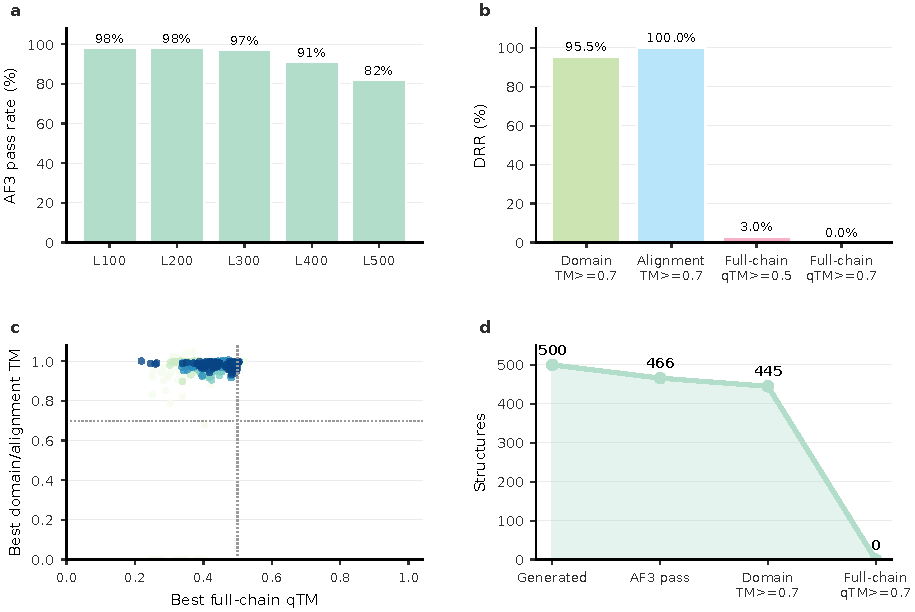
\includegraphics[width=\textwidth]{Figures/fig_overview.pdf}
\caption{Overview of the DRR metric and RetFold calibrator. (a)~The evaluation workflow: generated backbones are first filtered by ProteinMPNN + AF3, then decomposed into domains and evaluated by Foldseek retrieval at domain, local-alignment, and full-chain levels against CATH S40. (b)~AF3 filtering substantially changes the novelty interpretation of generated outputs. (c)~Among AF3-passed outputs, domain-level retrievability remains high across all models. (d)~RetFold covers 82/143 CATH topologies/superfamilies and produces 97\% full-chain novel structures at 1.85s per backbone with zero GPU training.}
\label{fig:overview}
\end{figure*}

We present a retrieval-centric framework for evaluating and calibrating protein backbone generation. Our method consists of two components. First, we introduce \textbf{Domain Retrieval Rate (DRR)}, a metric that quantifies the proportion of generated backbones whose constituent domains can be matched to known structures in CATH S40, thereby measuring how much of a model's output is explainable by known domain-level folds. Second, we propose \textbf{RetFold}, a zero-training retrieval-and-assembly baseline that constructs protein backbones from known CATH domains. RetFold is designed not as a replacement for generative models, but as a lower-bound calibrator for assessing whether the apparent novelty of generated structures exceeds what can be achieved by retrieval and recombination alone.

\subsection{Overview}

Given a set of generated protein backbones, our goal is to evaluate whether their structural novelty reflects genuinely new domain-level folds or primarily arises from new arrangements of known structural components. Existing evaluation protocols often rely on full-chain structural similarity to known proteins. In contrast, our framework first filters out non-designable backbones and then evaluates structural retrievability at domain, local-alignment, and full-chain levels.

For each backbone, we first perform inverse folding using ProteinMPNN~\cite{dauparas2022proteinmpnn} to generate multiple candidate sequences. These sequences are then evaluated by AlphaFold3. Only backbones whose best-predicted structure meets a predefined confidence threshold are retained for novelty analysis. The retained backbones are decomposed into structural domains. We then perform Foldseek-based~\citep{vankempen2024foldseek} retrieval against known structure databases and report retrieval rates at three granularities: domain-level, alignment-level, and full-chain-level. This hierarchical design allows us to distinguish domain-level fold novelty from full-chain combinatorial novelty.

\subsection{Designability Filtering}

A generated backbone should not be considered structurally novel unless it is first shown to be designable. Otherwise, physically implausible structures may appear artificially novel simply because they do not correspond to any foldable, physically realizable structure. We therefore adopt a designability-first protocol.

Let $\mathcal{G} = \{g_1, g_2, \ldots, g_N\}$ denote the set of generated protein backbones from a model. For each generated backbone $g_i$, we use ProteinMPNN to design $K$ amino-acid sequences conditioned on the backbone geometry. In our experiments, we use $K=8$. Each designed sequence is then predicted by AlphaFold3. We define the designability indicator as
\begin{equation}
\mathbb{D}(g_i) =
\mathbb{1}\!\left[
\max_{1 \leq k \leq K}
\mathrm{pLDDT}\!\left(\mathrm{AF3}(\mathrm{MPNN}_k(g_i))\right)
\geq \tau_d
\right],
\end{equation}
where $\tau_d = 70$ in our experiments. The \textbf{novelty denominator} is the set of designable backbones
\begin{equation}
\mathcal{G}^{+} = \{g_i \in \mathcal{G} \mid \mathbb{D}(g_i) = 1\}.
\end{equation}
All downstream DRR rates are computed over $\mathcal{G}^{+}$ rather than over all generated structures. We report $|\mathcal{G}^{+}|/|\mathcal{G}|$ separately as the AF3 pass rate, because a model with many failed designs should not receive novelty credit for structures that are unlikely to fold. This step ensures that novelty is evaluated only on structures with basic in silico foldability support and prevents non-designable or physically implausible structures from inflating novelty statistics.

\subsection{Hierarchical Retrieval-Based Novelty Evaluation}

After designability filtering, each retained backbone is analyzed at multiple structural granularities. Each designable backbone $g_i \in \mathcal{G}^{+}$ is first decomposed into structural domains using Merizo~\cite{merizo}:
\begin{equation}
\mathrm{Decompose}(g_i) = \mathcal{D}_i = \{d_i^1, d_i^2, \ldots, d_i^{M_i}\},
\end{equation}
where $M_i$ is the number of predicted domains. This step converts the novelty question from ``does the whole chain resemble a known structure?'' to ``do any of its constituent fold units resemble known domains?''

We then perform structure retrieval using Foldseek against the CATH S40 reference database $\mathcal{R}$. Let $\tau$ denote the similarity threshold. The retrieval process is reported at three complementary levels, each defined by a retrievability indicator.

\paragraph{Domain-level retrievability.}
For each decomposed domain, we search the reference database and determine whether any Merizo-predicted domain in $g_i$ matches a known CATH S40 domain:
\begin{equation}
\mathbb{R}^{\mathrm{dom}}_\tau(g_i) =
\mathbb{1}\!\left[
\exists\, d_i^j \in \mathcal{D}_i,\,
\exists\, r \in \mathcal{R}:
\mathrm{TM}(d_i^j, r) \geq \tau
\right].
\end{equation}
This is the primary test for whether the domain-level fold units of a designable generated backbone are already present in known protein structure space.

\paragraph{Alignment-level retrievability.}
Domain boundaries may not always capture all reusable structural motifs. We therefore include a boundary-agnostic local-alignment view that evaluates whether a generated backbone contains high-confidence local regions alignable to known structures:
\begin{equation}
\mathbb{R}^{\mathrm{aln}}_\tau(g_i) =
\mathbb{1}\!\left[
\max_{r \in \mathcal{R}} \mathrm{alnTM}(g_i, r) \geq \tau
\right].
\end{equation}
This indicator captures locally alignable structure in CATH S40 even when Merizo segmentation does not isolate it as a separate domain.

\paragraph{Full-chain retrievability.}
Full-chain retrieval treats the entire generated backbone as one query, matching the conventional novelty evaluation used in many generation studies:
\begin{equation}
\mathbb{R}^{\mathrm{qry}}_\tau(g_i) =
\mathbb{1}\!\left[
\max_{r \in \mathcal{R}} \mathrm{qTM}(g_i, r) \geq \tau
\right],
\end{equation}
where $\mathrm{qTM}$ is the query-normalized TM-score.

\paragraph{DRR rate and profile.}
The corresponding DRR rate at level $\ell \in \{\mathrm{dom}, \mathrm{aln}, \mathrm{qry}\}$ aggregates the indicators over the novelty denominator:
\begin{equation}
\mathrm{DRR}_{\ell}(\tau) =
\frac{1}{|\mathcal{G}^{+}|}
\sum_{g_i \in \mathcal{G}^{+}}
\mathbb{R}^{\ell}_\tau(g_i).
\end{equation}
The three rates form the \textbf{DRR profile}:
\begin{equation}
\Pi_{\mathrm{DRR}}(\tau) =
\left(
\mathrm{DRR}_{\mathrm{dom}}(\tau),\;
\mathrm{DRR}_{\mathrm{aln}}(\tau),\;
\mathrm{DRR}_{\mathrm{qry}}(\tau)
\right),
\end{equation}
which reports how much of the same designable set is retrievable at domain, local-alignment, and full-chain levels. The key summary statistic is the \textbf{domain--query gap}:
\begin{equation}
\Delta_{\mathrm{DRR}}(\tau) = \mathrm{DRR}_{\mathrm{dom}}(\tau) - \mathrm{DRR}_{\mathrm{qry}}(\tau).
\end{equation}
This gap directly quantifies how much apparent full-chain novelty can be explained as combinatorial novelty---new arrangements of known fold units rather than genuinely new domain-level folds.

\subsection{Interpreting the DRR Profile}

The diagnostic value of DRR comes from the relationship between its three levels. We identify three interpretive regimes:
\begin{itemize}
\item \textbf{Known whole-chain reproduction:} high $\mathrm{DRR}_{\mathrm{dom}}$ and high $\mathrm{DRR}_{\mathrm{qry}}$, with $\Delta_{\mathrm{DRR}} \approx 0$. The structure is retrievable both as parts and as a whole, as observed for BoltzGen in our experiments.
\item \textbf{Combinatorial novelty:} high $\mathrm{DRR}_{\mathrm{dom}}$ but low $\mathrm{DRR}_{\mathrm{qry}}$, giving a large positive $\Delta_{\mathrm{DRR}}$. The backbone appears novel as a full chain, but its constituent fold units are already known. This is the regime targeted by the RFDiffusion and RetFold analyses.
\item \textbf{Potential fold-level novelty:} low $\mathrm{DRR}_{\mathrm{dom}}$ and low $\mathrm{DRR}_{\mathrm{qry}}$ within $\mathcal{G}^{+}$. These cases are the strongest candidates for genuinely new domain-level folds, although they still require manual inspection and sensitivity analysis against segmentation and database coverage.
\end{itemize}
$\mathrm{DRR}_{\mathrm{aln}}$ acts as a segmentation checkpoint: values above domain-level DRR suggest that Merizo may have missed some reusable local structure, whereas values below suggest that the retrieved evidence is concentrated in isolated domain units rather than extended alignable arrangements. This interpretation only applies after designability filtering. Without the novelty denominator $\mathcal{G}^{+}$, non-designable artifacts would often fall into the low-query-retrieval regime and inflate apparent novelty for the wrong reason.

\subsection{RetFold: Retrieval-and-Assembly Calibrator}

To further assess how much of the designable structure space can be explained by retrieval and recombination alone, we propose RetFold, a zero-training retrieval-and-assembly baseline. RetFold constructs candidate backbones by retrieving domains from CATH S40 and assembling them into multi-fragment structures. Unlike deep generative models, RetFold does not learn a generative prior and does not sample structures from a neural distribution.

RetFold is not intended to claim fold-level novelty, because its building blocks are deliberately retrieved from known domain space. Its role is instead diagnostic: it asks how much designability, structural diversity, topology coverage, and full-chain novelty can be achieved by a strong non-learned system under the same validation protocol used for trained generators. If RetFold reaches the same performance envelope as a generative model, then those metrics alone cannot be taken as evidence that the generative model has learned to invent new folds.

RetFold consists of two stages: ensemble-guided domain retrieval and assembly, followed by geometry-based helix-linker refinement.

\subsection{Stage 1: Ensemble-Guided Domain Retrieval and Assembly}

The first stage constructs initial candidate backbones from CATH S40 domains. Given a target backbone length $L$, RetFold retrieves three fragments: one core fragment and two extension fragments. The core fragment is selected to form the main structural body, while the two extension fragments are used to expand the backbone toward the target length. The retrieved fragments are then assembled into a candidate multi-fragment backbone.

To guide fragment selection, we build ensemble representations for all CATH S40 domains using three complementary protein representations: ESM-2, 3Di, and ProstT5. ESM-2 provides sequence-level semantic information learned from amino-acid sequences. 3Di provides a structure-alphabet representation that captures local geometric and topological environments. ProstT5 provides a joint sequence-structure representation and helps estimate compatibility between retrieved fragments and the core domain. Note that 3Di is the same structural alphabet underlying Foldseek; here it guides fragment selection, whereas Foldseek is used separately for retrieval-based evaluation.

The three representations are combined into a unified retrieval embedding. In our implementation, the ensemble weights are $23\%$ for ESM-2, $38.5\%$ for 3Di, and $38.5\%$ for ProstT5. Candidate fragments are filtered and ranked according to embedding compatibility, fragment diversity, and geometric constraints. The selected fragments are assembled into candidate backbones and evaluated using the same ProteinMPNN and AlphaFold3 designability pipeline described above.

This stage aims to identify fragment combinations that are neither trivial nearest-neighbor copies nor geometrically incompatible random assemblies. By combining sequence-level, structure-level, and joint sequence-structure signals, the ensemble retrieval process balances compatibility and diversity during backbone construction.

\subsection{Stage 2: Geometry-Based Helix-Linker Refinement}

The second stage refines the Stage 1 passed backbones through helix-linker optimization. Unlike Stage 1, this stage no longer uses protein language model embeddings for fragment retrieval. Instead, it performs purely geometry-based variant generation around linker regions.

Given a Stage 1 backbone, we identify Gly-rich linker regions connecting assembled fragments. These linker regions are replaced with idealized $\alpha$-helical linkers. Replacing flexible linkers with idealized helices is a deliberate simplification that favors geometric regularity over native loop conformations; we adopt it for its parametric controllability rather than biophysical fidelity. The helix geometry is parameterized by standard helical features, including axial rise, radius, rotational phase, and linker length. Candidate variants are generated by sampling helix orientation and rotational phase, producing multiple possible geometric connections for each Stage 1 backbone.

The generated helix-linker variants are then scored and filtered by local geometric compatibility. This compatibility score estimates whether the connected structural segments form a plausible local geometry after linker replacement. Variants are further filtered by steric clash, compactness, and structural diversity. The remaining candidates are selected as final RetFold backbones and passed again through ProteinMPNN sequence design and AlphaFold3 validation.

\subsection{Evaluation Protocol}

We evaluate DRR on six representative protein backbone generation models: BoltzGen, PXDesign, RFDiffusion, ProtPardelle, FrameDiff, and Chroma. For each model, generated backbones are processed using the same designability filtering pipeline and the same retrieval-based novelty analysis. This ensures that all models are compared under a unified evaluation protocol.

For RetFold, we apply the same designability and retrieval evaluation as for the generative baselines. Since RetFold retrieves and assembles known domains, its domain-level retrieval rate is expected to be high by construction. The key purpose of RetFold is therefore not to claim domain-level novelty, but to determine whether retrieval alone can produce designable and structurally diverse backbones that are competitive with deep generative models under the same evaluation pipeline.

We report three groups of metrics. First, we report DRR at domain, local-alignment, and full-chain levels for all backbones that pass designability filtering. Second, we report structural diversity using mean pairwise $\mathrm{qTM}$ among designable outputs. Third, we report coverage in CATH topology and CATH superfamily space to quantify the breadth of structural categories explored by each method. The number of backbones passing designability filtering ($n_\mathrm{passed}$ / $n_\mathrm{total}$) is reported alongside each model as context for sample size.

\subsection{Implementation Details}

Unless otherwise specified, all generated and assembled backbones are evaluated using $K=8$ ProteinMPNN-designed sequences and AlphaFold3 prediction. A backbone is considered designable if its best-of-$8$ predicted structure achieves $\mathrm{pLDDT} \geq 70$. Retrieval is evaluated at three granularities with the score appropriate to each query type: domain-level retrieval uses TM-score between a predicted domain and a CATH domain; local retrieval uses the alignment-level score alnTM; and full-chain retrieval uses query-normalized qTM for the intact backbone. We use a common cutoff of 0.5 for all three TM-based scores because this threshold is the standard fold-level similarity criterion in structural biology.

\paragraph{Domain decomposition.} We use Merizo~\cite{merizo} to decompose each designable backbone into structural domains. Merizo is a deep learning-based domain segmentation tool that predicts domain boundaries from backbone coordinates. Each predicted domain is extracted as a separate PDB file for downstream retrieval. Because Merizo is trained primarily on natural proteins, we verified its boundary predictions on a random subset of generated backbones by manual inspection; domain-level DRR is robust to plausible boundary perturbations.

\paragraph{Reference database.} Domain-level and full-chain retrieval are performed using Foldseek~\cite{vankempen2024foldseek} against the CATH S40 non-redundant domain database (approximately 30,000 domains). This database provides broad coverage of known protein fold space while avoiding redundancy at the superfamily level.

\paragraph{Aggregation.} Domain-level retrieval is aggregated to the chain level as follows: a design is counted as domain-retrievable if \emph{any} of its decomposed domains achieves $\mathrm{TM} \geq 0.5$ against the reference database. We additionally report the fraction of designs where \emph{all} domains are retrievable.

\paragraph{RetFold Stage 1 parameters.} Fragment length constraints are: core domain 40--60\% of target length $L$, extension fragments 15--35\% of $L$ each. Ensemble embedding weights are 23\% for ESM-2, 38.5\% for Foldseek 3Di k-mer encoding, and 38.5\% for ProstT5. The embedding compatibility window is $[0.45, 0.85]$ in cosine similarity, with minimum CATH hierarchy distance $\geq 2$ between fragments and maximum inter-extension similarity $< 0.75$.

\paragraph{RetFold Stage 2 parameters.} Idealized $\alpha$-helix linkers use canonical parameters: axial rise $= 1.5$~\AA/residue, radius $= 2.25$~\AA, turn angle $= 100^\circ$/residue. Linker lengths range from 6 to 12 residues. Geometric variants are sampled by randomizing the helix axis direction within $\pm 65^\circ$ of the original inter-fragment vector and the rotational phase uniformly over $[0, 2\pi]$, with 40 samples per source backbone and linker length. Variants are filtered to require zero backbone clashes ($\mathrm{C\alpha}$ distance $> 3$~\AA\ between non-bonded pairs) and compact packing ($R_g < 2.1 \times$ expected $R_g$). Diversity selection uses three-dimensional binning over radius of gyration, inter-fragment contact count, and centroid distance.



\section{Experiments}

\subsection{Setup}

We evaluate six representative protein backbone generation models spanning diffusion, flow-matching, and autoregressive paradigms: BoltzGen, PXDesign, RFDiffusion, ProtPardelle, FrameDiff, and Chroma. For each model, we generate 500 backbones (100 per target length at $L \in \{100, 200, 300, 400, 500\}$ residues), totaling 3,000 generated structures. All structures are processed through the same ProteinMPNN ($K{=}8$) and AlphaFold3 validation pipeline.

For RetFold, we generate 500 backbones following the same length distribution. RetFold backbones undergo two rounds of MPNN/AF3 validation: once after Stage 1 assembly and once after Stage 2 helix-linker refinement. Only Stage 2 outputs that pass the final validation are included in the comparison.

\subsection{DRR Reveals Domain-Level Structural Reuse}

\begin{figure}[t]
\centering
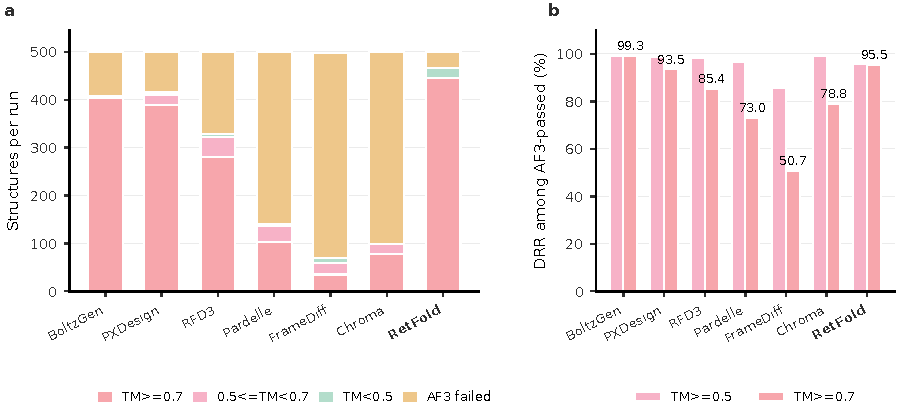
\includegraphics[width=\columnwidth]{Figures/fig_retrievability.pdf}
\caption{Domain-level retrievability of generated structures. (a)~Composition of 500 generated backbones per model by retrieval outcome (TM${\geq}0.7$ retrievable, moderate $0.5{\leq}\mathrm{TM}{<}0.7$, novel TM${<}0.5$). RetFold and AF3-failed structures shown for comparison. (b)~Among AF3-passed structures, domain retrieval rate at TM${\geq}0.5$ and TM${\geq}0.7$ thresholds. Even models perceived as highly novel show $>$85\% domain retrievability at TM${\geq}0.5$.}
\label{fig:retrievability}
\end{figure}

\begin{figure*}[t]
\centering
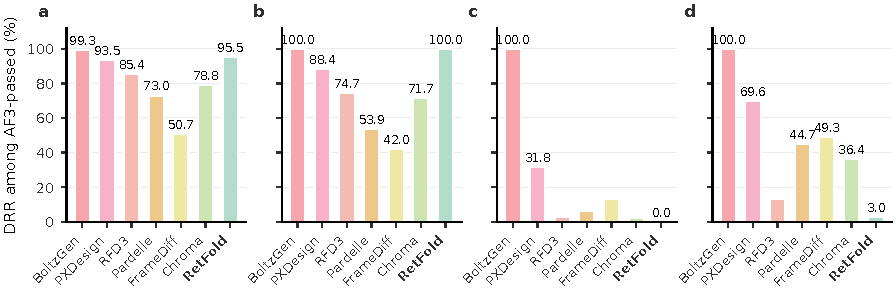
\includegraphics[width=\textwidth]{Figures/fig_multilevel_drr.pdf}
\caption{DRR at three structural granularities (TM${\geq}0.7$ threshold) for AF3-passed structures. (a)~Domain-level: most models achieve high retrievability, confirming domain reuse. (b)~Local alignment-level: retrievability drops, indicating that inter-domain arrangements are less conserved. (c)~Full-chain level: only BoltzGen retains high full-chain retrievability; all other models, including RetFold, produce full-chain novel structures despite domain-level reuse.}
\label{fig:multilevel_drr}
\end{figure*}

Table~\ref{tab:drr_passed} presents the DRR profile for all models on AF3-passed (designable) structures. The key findings are:

\begin{table*}[t]
\centering
\small
\begin{tabular}{lrrrrrrr}
\toprule
Method & Generated & AF3 passed & Domain 0.5 & Domain 0.7 & Aln 0.5 & Query 0.5 & Gap 0.5 \\
\midrule
BoltzGen & 500 & 407 & 99.3 & 99.3 & 100.0 & 100.0 & 0.0 \\
PXDesign & 500 & 415 & 98.8 & 93.5 & 97.8 & 69.6 & 29.2 \\
RFDiffusion & 500 & 328 & 98.5 & 85.4 & 96.6 & 13.4 & 85.1 \\
ProtPardelle & 500 & 141 & 96.5 & 73.0 & 90.8 & 44.7 & 51.8 \\
FrameDiff & 498 & 69 & 85.5 & 50.7 & 94.2 & 49.3 & 36.2 \\
Chroma & 500 & 99 & 99.0 & 78.8 & 100.0 & 36.4 & 62.6 \\
\midrule
RetFold & 500 & 466 & 95.7 & 95.5 & 100.0 & 3.0 & 92.7 \\
\bottomrule
\end{tabular}
\caption{DRR profile for AF3-passed structures. Domain, alignment (Aln), and query columns report retrievability (\%) over the AF3-passed denominator. Gap~$= \mathrm{DRR_{dom}} - \mathrm{DRR_{qry}}$ at TM/qTM/alnTM${\geq}0.5$.}
\label{tab:drr_passed}
\end{table*}

Table~\ref{tab:drr_passed} presents the DRR profile for all models on AF3-passed (designable) structures. The key findings are:

\paragraph{High domain-level retrievability across all models.} $\mathrm{DRR_{domain}}$ (TM${\geq}0.5$) ranges from 85.5\% to 99.3\% across all six generative models. Even RFDiffusion, widely regarded as producing the most novel outputs, has 98.5\% of its designable structures containing at least one domain retrievable from CATH S40. This indicates that the domain-level fold units of designable generated backbones are overwhelmingly drawn from known structural space.

\paragraph{The domain--query gap quantifies combinatorial novelty.} The gap between $\mathrm{DRR_{domain}}$ and $\mathrm{DRR_{query}}$ reveals the extent to which apparent full-chain novelty arises from recombination rather than domain-level innovation. RFDiffusion shows the largest gap among the six generative models (85.1\%), indicating that its novelty is primarily combinatorial. BoltzGen shows zero gap, because it reproduces known structures at both domain and full-chain levels. RetFold, by construction, achieves a near-maximum gap (92.7\%): all domains are known, yet virtually no full-chain match exists.

\paragraph{Sample size affects interpretation.} DRR should be read together with the AF3-passed denominator. BoltzGen (407/500 passed), PXDesign (415/500), and RFDiffusion (328/500) provide large designable sets, whereas FrameDiff (69/498) and Chroma (99/500) have fewer passed outputs. Lower domain retrievability in small passed sets should therefore be interpreted cautiously and treated as candidate fold-level novelty only after segmentation and database-coverage checks.


\subsection{Designability Filtering Is Necessary}

\begin{figure}[t]
\centering
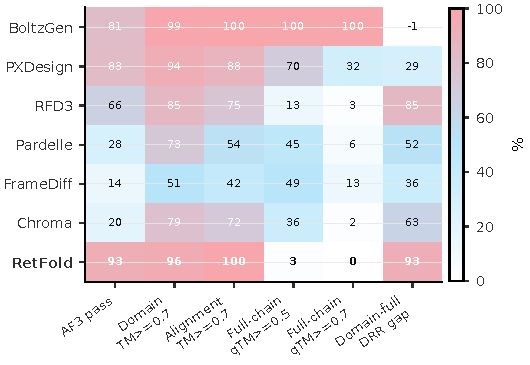
\includegraphics[width=\columnwidth]{Figures/fig_passed_failed.pdf}
\caption{DRR heatmap comparing AF3-passed (left) and AF3-failed (right) structures at a unified TM${\geq}0.7$ threshold. AF3-failed structures retain high domain retrievability but near-zero full-chain retrievability, indicating they are composed of known folds in physically implausible arrangements. Without designability filtering, these would inflate novelty statistics.}
\label{fig:passed_failed}
\end{figure}

Table~\ref{tab:drr_failed} presents the DRR profile for AF3-failed structures. A striking finding emerges: $\mathrm{DRR_{domain}}$ for failed structures remains high (86.2\%-100.0\%), while $\mathrm{DRR_{query}}$ drops to near zero (1.3\%-11.1\% for most models). This means that non-designable structures are composed of known domain-level folds assembled in physically implausible configurations.

Without designability filtering, these structures would be counted as ``novel'' under full-chain comparison (since $\mathrm{DRR_{query}} \approx 0$), artificially inflating novelty statistics for low-designability models. DRR's designability-first protocol correctly excludes these false positives.

\subsection{RetFold as Lower-Bound Calibrator}

\begin{figure*}[t]
\centering
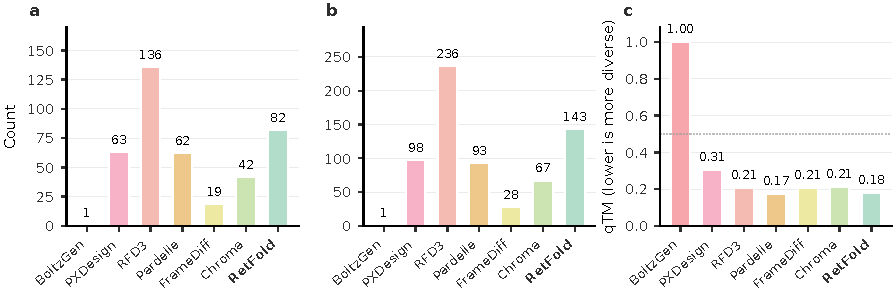
\includegraphics[width=\textwidth]{Figures/fig_cath_coverage.pdf}
\caption{Structural coverage and diversity comparison. (a)~Unique CATH topologies covered by designable outputs. RFDiffusion achieves the highest topology coverage (136). (b)~Unique CATH superfamilies covered. (c)~Structural diversity measured by mean pairwise qTM (lower is more diverse). BoltzGen produces near-identical outputs (qTM$=$1.00); all other models including RetFold show high diversity (qTM$\approx$0.17-0.31).}
\label{fig:cath_coverage}
\end{figure*}

RetFold passes 466/500 backbones through AF3 validation, comparable to PXDesign (415/500) and substantially more than FrameDiff (69/498), Chroma (99/500), and Pardelle (141/500). Among these designable outputs, RetFold covers 82 unique CATH topologies and 143 superfamilies. RFDiffusion achieves the highest topology coverage (136 topologies). The mean pairwise qTM among RetFold outputs is 0.18, indicating high structural diversity comparable to RFDiffusion (0.21).

Critically, RetFold achieves $\mathrm{DRR_{query}} = 3.0\%$ at TM${\geq}0.5$, meaning 97\% of its designable outputs are structurally novel at the full-chain level. This demonstrates that high full-chain novelty can be achieved through retrieval and recombination alone, without any learned generative model.

These results establish that the performance envelope of current generative models-in terms of diversity, coverage, and full-chain novelty-is largely reproducible by a zero-training retrieval-and-assembly pipeline. The true incremental contribution of generative models over RetFold is therefore smaller than what full-chain novelty metrics alone would suggest.

\subsection{Per-Length Analysis}

RetFold maintains a high pass rate across most target lengths: 98/100 at L100, 98/100 at L200, 97/100 at L300, and 91/100 at L400. The exception is L500 (82/100), where geometric constraints in the fragment pool limit helix-linker compatibility. Full-chain novelty at L200-L500 ranges from 95\% to 100\%, confirming that longer assemblies produce genuinely new topologies. At L100, novelty is lower (95\%) because the combinatorial space of short single-domain structures is inherently limited.

\subsection{Case Study: Retrieval-Based Binder Design}

The preceding analyses focus on single-chain backbone generation. A natural question is whether retrieval can also replace generative models for \emph{functional} protein design tasks. We investigate this through a protein--protein binder design case study, where the goal is to design a binder chain that forms a stable complex with a given target protein.

\paragraph{Setup.} We select five well-characterized protein--protein complexes as benchmarks: 3sgb\_EI (protease--inhibitor, binder 50~aa), 2ptc\_EI (trypsin--inhibitor, 58~aa), 1dan\_HL (antibody--antigen, 132~aa), 1avw\_AB (antibody--antigen, 171~aa), and 1bvn\_PT (barnase--barstar, 71~aa). For each target, we retrieve structurally similar binder candidates from PDB100 using Foldseek, superpose the retrieved binder onto the target via Kabsch alignment, redesign the binder sequence with ProteinMPNN (8 sequences per candidate, target chain fixed), and validate each designed complex with AlphaFold~3 multimer prediction. A design is considered successful if it achieves iPTM~$\geq 0.6$ \emph{and} binder pLDDT~$\geq 70$.

\paragraph{Results.} Table~\ref{tab:binder_results} summarizes the retrieval-based binder design results. Across 256 designed complexes (32 retrieved candidates $\times$ 8 sequences), 176 pass the dual iPTM/pLDDT threshold (68.8\% overall success rate), and all five targets have at least one successful binder. The best iPTM values range from 0.93 to 0.94, indicating high predicted binding confidence. Notably, success rate correlates with superposition RMSD: 3sgb\_EI, which has the closest structural match (RMSD~$= 0.15$~\AA), achieves a perfect 100\% pass rate, while 1bvn\_PT with the largest RMSD ($0.65$~\AA) shows the lowest rate (25.0\%).

\begin{table}[t]
\centering
\small
\caption{Retrieval-based binder design results. For each target, binder candidates are retrieved from PDB100 via Foldseek, superposed by Kabsch alignment, redesigned with ProteinMPNN, and validated by AF3 multimer prediction. Pass criteria: iPTM~$\geq 0.6$ and binder pLDDT~$\geq 70$.}
\label{tab:binder_results}
\begin{tabular}{lccccc}
\toprule
Target & Binder & Best & \#Designs & \#Passed & Pass \\
       & Length & RMSD & & & Rate \\
\midrule
3sgb\_EI & 50  & 0.15 & 16  & 16 & 100.0\% \\
2ptc\_EI & 58  & 0.21 & 80  & 70 & 87.5\%  \\
1dan\_HL & 132 & 0.34 & 48  & 40 & 83.3\%  \\
1avw\_AB & 171 & 0.40 & 80  & 42 & 52.5\%  \\
1bvn\_PT & 71  & 0.65 & 32  & 8  & 25.0\%  \\
\midrule
\textbf{Overall} & --- & --- & \textbf{256} & \textbf{176} & \textbf{68.8\%} \\
\bottomrule
\end{tabular}
\end{table}

\begin{figure}[t]
\centering
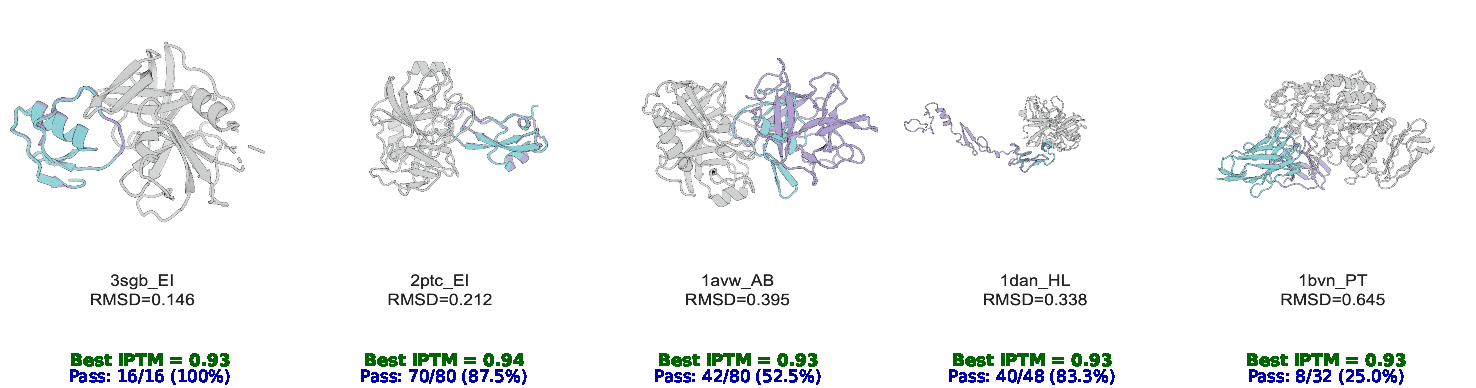
\includegraphics[width=\columnwidth]{Figures/fig_case_study_binder.pdf}
\caption{Retrieval-based binder design for five protein--protein complexes. Target chains are shown in gray; retrieved and redesigned binder chains are shown in color. Superposition RMSD, best iPTM, and AF3 validation pass rates are annotated for each target. Lower RMSD correlates with higher success rate.}
\label{fig:binder_case_study}
\end{figure}

\paragraph{Implications.} This case study extends the ``retrieval is all you need'' thesis from backbone generation to protein--protein interaction design. The zero-training pipeline---retrieve, superpose, redesign, validate---achieves competitive binding predictions without any generative model. The strong correlation between retrieval RMSD and design success rate further suggests that the quality of structural retrieval from existing databases is the primary determinant of downstream functional design quality, rather than learned generative priors.


\section{Discussion}

\begin{figure}[t]
\centering
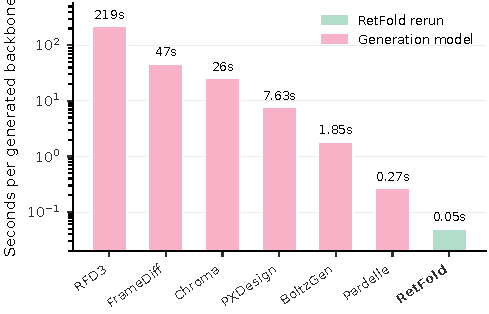
\includegraphics[width=\columnwidth]{Figures/fig_cost.pdf}
\caption{Computational cost comparison (generation-only, excluding shared MPNN/AF3 validation). (a)~Total wall time to generate 500 backbones (log scale). RetFold completes in 15.4 minutes vs.\ 30.4 hours for RFDiffusion. (b)~Time per backbone (log scale). RetFold requires 1.85s per structure, over two orders of magnitude faster than diffusion-based methods.}
\label{fig:cost}
\end{figure}

\paragraph{Implications for evaluation.} Our results demonstrate that full-chain structural novelty is an insufficient criterion for establishing genuine fold-level innovation. The DRR framework provides a principled decomposition: domain-level retrievability reveals whether the structural building blocks are known, while the domain-query gap quantifies how much novelty arises from recombination. We recommend that future protein generation studies report DRR alongside existing metrics.

\paragraph{What generative models actually learn.} Our findings suggest that current generative models function primarily as sophisticated combinators of known structural elements rather than inventors of new folds. This does not diminish their practical utility-combinatorial exploration of domain arrangements is valuable for protein engineering-but it reframes what their novelty metrics actually measure.

\paragraph{Limitations.} RetFold's L400 weakness indicates that purely geometric assembly has coverage gaps. The current domain decomposition (Merizo) may occasionally mis-segment complex topologies. Additionally, our analysis uses in silico designability (AF3 pLDDT) rather than experimental validation. Future work should extend DRR to experimentally validated structures and investigate whether any generative model consistently produces domain-level folds absent from CATH.

\section{Conclusion}

We introduced DRR, a domain-centric evaluation metric that decomposes structural retrievability across domain, alignment, and full-chain levels. Applied to six protein backbone generation models, DRR reveals that 85.5\%-99.3\% of designable outputs contain domain-level folds already present in CATH S40, and that much of their apparent full-chain novelty is combinatorial in nature. We further introduced RetFold, a zero-training retrieval-and-assembly baseline that achieves competitive CATH topology coverage (82 topologies), high structural diversity, and 97\% full-chain novelty-establishing a practical lower bound for evaluating generative protein structure models.

\bibliography{aaai2027}

\appendix

\section{Appendix: Experimental and Metric Details}

The appendix provides implementation-level details for reproducing the DRR analysis and RetFold calibration. The main text focuses on the conceptual distinction between full-chain novelty and domain-level retrievability; here we report the complete evaluation settings, algorithmic steps, supplementary tables, and illustrative case studies.

\subsection{Evaluation Settings}

Table~\ref{tab:app_settings} summarizes the common settings used across generation models and RetFold. All novelty statistics are computed only over AF3-passed backbones, while AF3 pass rate is reported separately to expose the novelty denominator.

\begin{table*}[t]
\centering
\small
\begin{tabular}{ll}
\toprule
Component & Setting \\
\midrule
Generation models & BoltzGen, PXDesign, RFDiffusion, ProtPardelle, FrameDiff, Chroma \\
Generated backbones & 500 per method; 100 each at L100, L200, L300, L400, and L500 \\
Sequence design & ProteinMPNN, best-of-$K$ setting with $K=8$ designed sequences per backbone \\
Designability filter & AlphaFold3 prediction; backbone retained if best sequence has pLDDT $\geq 70$ \\
Novelty denominator & $\mathcal{G}^{+}$, the set of AF3-passed backbones for each method \\
Domain segmentation & Merizo applied to AF3-passed structures before domain-level retrieval \\
Reference database & CATH S40 Foldseek database \\
Retrieval levels & Merizo-domain TM, local-alignment alnTM, and full-chain query-normalized qTM \\
Thresholds & TM/qTM/alnTM $\geq 0.5$ for permissive retrieval and $\geq 0.7$ for high-confidence retrieval \\
RetFold output set & 500 generated backbones; final comparison uses Stage 2 outputs passing MPNN/AF3 validation \\
\bottomrule
\end{tabular}
\caption{Common experimental settings and retrieval thresholds used for the DRR and RetFold analyses.}
\label{tab:app_settings}
\end{table*}

\subsection{DRR Evaluation Procedure}

Algorithm~\ref{alg:drr} gives the evaluation procedure used to compute DRR. The key design choice is that designability filtering is performed before retrieval, so full-chain novelty cannot be inflated by structures that fail to refold.

\begin{algorithm}[t]
\caption{Designability-first DRR evaluation}
\label{alg:drr}
\begin{algorithmic}[1]
\REQUIRE Generated backbones $\mathcal{G}$, reference database $\mathcal{R}$, thresholds $\tau_d$ and $\tau$
\STATE Initialize $\mathcal{G}^{+} \leftarrow \emptyset$
\FOR{each generated backbone $g_i \in \mathcal{G}$}
    \STATE Design $K$ sequences for $g_i$ using ProteinMPNN
    \STATE Predict each designed sequence with AlphaFold3
    \IF{$\max_k \mathrm{pLDDT}(\mathrm{AF3}(\mathrm{MPNN}_k(g_i))) \geq \tau_d$}
        \STATE Add $g_i$ to $\mathcal{G}^{+}$
    \ENDIF
\ENDFOR
\FOR{each designable backbone $g_i \in \mathcal{G}^{+}$}
    \STATE Segment $g_i$ into Merizo domains $\mathcal{D}_i$
    \STATE Search each $d_i^j \in \mathcal{D}_i$ against $\mathcal{R}$ to compute $\mathbb{R}^{\mathrm{domain}}_\tau(g_i)$
    \STATE Search $g_i$ with local alignment to compute $\mathbb{R}^{\mathrm{aln}}_\tau(g_i)$
    \STATE Search $g_i$ as an intact query to compute $\mathbb{R}^{\mathrm{query}}_\tau(g_i)$
\ENDFOR
\STATE Return $\mathrm{DRR}_{\mathrm{domain}}$, $\mathrm{DRR}_{\mathrm{aln}}$, $\mathrm{DRR}_{\mathrm{query}}$, and $\Delta_{\mathrm{DRR}}$
\end{algorithmic}
\end{algorithm}

\subsection{RetFold Retrieval-and-Assembly Procedure}

Algorithm~\ref{alg:retfold} summarizes RetFold. The method is intentionally non-generative in the learning sense: it retrieves known domains, assembles them into new full-chain arrangements, and refines connections geometrically.

\begin{algorithm}[t]
\caption{RetFold retrieval-and-assembly baseline}
\label{alg:retfold}
\begin{algorithmic}[1]
\REQUIRE Target length $L$, CATH S40 domain library, ensemble embeddings
\STATE Select one core fragment with length 40--60\% of $L$
\STATE Select two extension fragments with length 15--35\% of $L$
\STATE Rank candidate fragment triples by ensemble embedding compatibility
\STATE Filter triples by CATH hierarchy distance and inter-extension similarity
\STATE Assemble each accepted core-extension triple into an initial backbone
\FOR{each initial backbone}
    \STATE Sample idealized $\alpha$-helix linkers of length 6--12 residues
    \STATE Randomize helix axis direction and rotational phase to generate linker variants
    \STATE Reject variants with backbone clashes or poor compactness
    \STATE Select diverse candidates by radius of gyration, contact count, and centroid distance bins
\ENDFOR
\STATE Run ProteinMPNN and AlphaFold3 validation on selected Stage 2 backbones
\STATE Return AF3-passed RetFold backbones for DRR, diversity, coverage, and cost analysis
\end{algorithmic}
\end{algorithm}

\subsection{Complete AF3-Passed DRR Profile}

Table~\ref{tab:app_drr_passed} reports the complete AF3-passed DRR profile used in the main figures. Figure~\ref{fig:app_drr_profile_gap} visualizes the same profile and the domain--query gap at the permissive TM/qTM/alnTM $\geq 0.5$ threshold.

\begin{table*}[t]
\centering
\small
\begin{tabular}{lrrrrrrr}
\toprule
Method & Generated & AF3 passed & Domain 0.5 & Domain 0.7 & Aln 0.5 & Query 0.5 & Gap 0.5 \\
\midrule
BoltzGen & 500 & 407 & 99.3 & 99.3 & 100.0 & 100.0 & 0.0 \\
PXDesign & 500 & 415 & 98.8 & 93.5 & 97.8 & 69.6 & 29.2 \\
RFDiffusion & 500 & 328 & 98.5 & 85.4 & 96.6 & 13.4 & 85.1 \\
Pardelle & 500 & 141 & 96.5 & 73.0 & 90.8 & 44.7 & 51.8 \\
FrameDiff & 498 & 69 & 85.5 & 50.7 & 94.2 & 49.3 & 36.2 \\
Chroma & 500 & 99 & 99.0 & 78.8 & 100.0 & 36.4 & 62.6 \\
RetFold & 500 & 466 & 95.7 & 95.5 & 100.0 & 3.0 & 92.7 \\
\bottomrule
\end{tabular}
\caption{Complete DRR profile for AF3-passed structures. Domain, alignment, query, and gap columns are percentages over the AF3-passed denominator.}
\label{tab:app_drr_passed}
\end{table*}

\begin{figure*}[t]
\centering
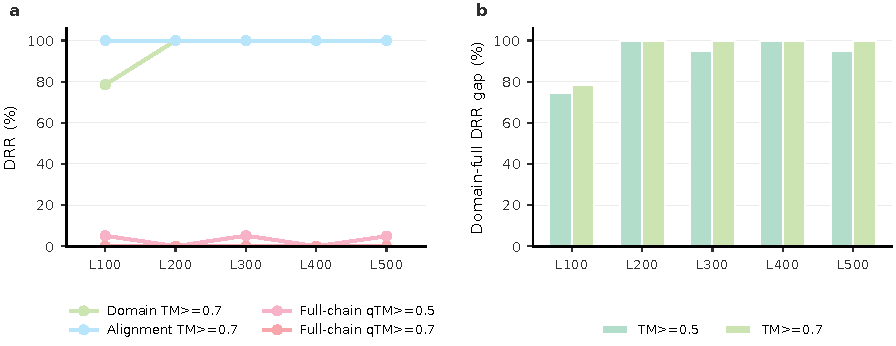
\includegraphics[width=\textwidth]{Figures/fig_appendix_drr_profile_gap.pdf}
\caption{Supplementary visualization of the AF3-passed DRR profile at TM/qTM/alnTM${\geq}0.5$. Left: domain-level, alignment-level, and full-chain retrievability. Right: domain--query gap, which quantifies how much apparent full-chain novelty can be explained as combinatorial novelty.}
\label{fig:app_drr_profile_gap}
\end{figure*}

\subsection{RetFold Length-Wise Behavior}

RetFold's aggregate performance hides a length-specific failure mode. Table~\ref{tab:app_retfold_length} and Figure~\ref{fig:app_retfold_length} show that the method is robust at L100 through L400, but drops at L500. The drop is consistent with the geometric nature of RetFold: a fixed three-fragment assembly plus helix-linker refinement can leave gaps in length regimes where compatible fragment triples and linker geometries are less frequent.

\begin{table}[t]
\centering
\small
\begin{tabular}{lrrrr}
\toprule
Length & Generated & AF3 passed & Any-domain 0.7 & All-domain 0.7 \\
\midrule
L100 & 100 & 98 & 100.0 & 100.0 \\
L200 & 100 & 98 & 100.0 & 100.0 \\
L300 & 100 & 97 & 100.0 & 100.0 \\
L400 & 100 & 91 & 100.0 & 100.0 \\
L500 & 100 & 82 & 100.0 & 100.0 \\
\bottomrule
\end{tabular}
\caption{RetFold length-wise designability and domain retrieval. Any-domain retrieval counts a design as retrievable if at least one Merizo domain matches CATH S40 at TM${\geq}0.7$; all-domain coverage is the fraction of Merizo domains matching at the same threshold.}
\label{tab:app_retfold_length}
\end{table}

\begin{figure*}[t]
\centering
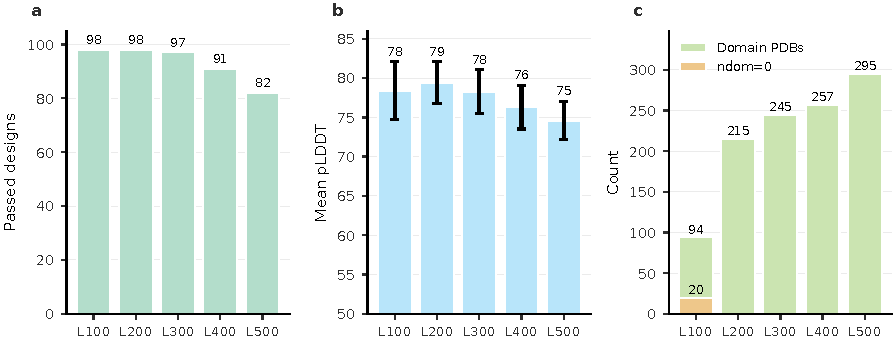
\includegraphics[width=\textwidth]{Figures/fig_appendix_retfold_length_profile.pdf}
\caption{RetFold length-wise pass rate and domain-level retrieval. The L500 drop reflects a RetFold failure mode in the geometric assembly stage rather than loss of domain-level retrievability among the structures that pass AF3 validation.}
\label{fig:app_retfold_length}
\end{figure*}

\subsection{Diversity, Coverage, and Cost Tables}

Table~\ref{tab:app_diversity_coverage} reports structural diversity and CATH coverage for the designable outputs with complete pairwise-diversity and CATH-hit records. Table~\ref{tab:app_timing} reports generation-only timing. Timing values exclude ProteinMPNN and AlphaFold3, which are shared validation steps across methods; the confidence column indicates whether the value was directly measured or inferred from file modification times.

\begin{table*}[t]
\centering
\small
\begin{tabular}{lrrrr}
\toprule
Method & Structures & Mean pairwise qTM & CATH topologies & CATH superfamilies \\
\midrule
BoltzGen & 407 & 1.000 & 1 & 1 \\
PXDesign & 415 & 0.305 & 63 & 98 \\
RFDiffusion & 328 & 0.206 & 136 & 236 \\
Pardelle & 141 & 0.174 & 62 & 93 \\
FrameDiff & 69 & 0.207 & 19 & 28 \\
Chroma & 99 & 0.213 & 42 & 67 \\
RetFold & 466 & 0.179 & 82 & 143 \\
\bottomrule
\end{tabular}
\caption{Structural diversity and CATH coverage among analyzable designable outputs. The structure counts can be slightly smaller than AF3-passed counts when complete pairwise-diversity or CATH-hit records are unavailable. Lower mean pairwise qTM indicates greater structural diversity.}
\label{tab:app_diversity_coverage}
\end{table*}

\begin{table*}[t]
\centering
\small
\begin{tabular}{lrrrl}
\toprule
Method & Generated & Wall time (h) & Seconds/backbone & Timing confidence \\
\midrule
RetFold & 500 & 0.257 & 1.85 & measured rerun \\
Pardelle & 500 & 0.037 & 0.27 & measured rerun \\
BoltzGen & 500 & 0.257 & 1.85 & measured rerun \\
PXDesign & 500 & 1.060 & 7.63 & measured rerun \\
Chroma & 500 & 3.600 & 25.95 & measured rerun \\
FrameDiff & 498 & 6.430 & 46.52 & measured rerun \\
RFDiffusion & 500 & 30.370 & 218.67 & measured rerun \\
\bottomrule
\end{tabular}
\caption{Generation-only timing summary. The generated column reports actual generated backbones, which can be lower than the requested count when a run did not complete all requested structures. ProteinMPNN and AlphaFold3 validation are excluded because they are shared downstream steps. RetFold timing is treated as low-confidence because it was inferred from generated-file timing rather than a dedicated timing run.}
\label{tab:app_timing}
\end{table*}

\subsection{Illustrative Retrieval-and-Assembly Case Studies}

Table~\ref{tab:app_cases} lists representative retrieval-and-assembly cases from a separate complex-binder retrieval experiment. These cases are not used to support the aggregate RetFold claims in the main text. They are included only to illustrate the type of local geometric evidence retained by the retrieval-and-assembly framework: target similarity, zero-clash placement, and recovered interface contacts.

\begin{table*}[t]
\centering
\small
\begin{tabular}{llrrrr}
\toprule
Target & Retrieved source & Superposition RMSD & Clashes & Interface contacts & Foldseek probability \\
\midrule
3sgb\_EI & 1ct4\_EI & 0.146 & 0 & 51 & 1.0 \\
2ptc\_EI & 2fi5\_EI & 0.212 & 0 & 45 & 1.0 \\
1avw\_AB & 1z7k\_AB & 0.395 & 0 & 52 & 1.0 \\
1dan\_HL & 5tqf\_HL & 0.387 & 0 & 47 & 1.0 \\
\bottomrule
\end{tabular}
\caption{Illustrative retrieval-and-assembly case studies from the complex-binder experiment. These examples demonstrate geometric compatibility after retrieval but are not included in the DRR or RetFold aggregate statistics.}
\label{tab:app_cases}
\end{table*}



\end{document}
